%\section{Parareal Stopping Criterion}
%
%\begin{frame}{Parareal Stopping Criterion}
%  \begin{itemize}
%    \item
%      \texttt{nconverged} successive iterations without significant change:
%      \begin{equation}
%        \tag{7.5}
%        \norm{U_n^k - U_n^{k-1}} \leq \epsilon\max\Set[\big]{
%        \norm{U_n^k}, \norm{U_n^{k-1}}
%        }
%      \end{equation}
%    \item
%      all previous stages must have converged
%
%      (experiments with Van der Pol oscillator: divergence looks like convergence $\implies$ late parareal stages falsly converge)
%
%      \url{https://gitlab.mpi-magdeburg.mpg.de/jschulze/ParaReal.jl/-/issues/3\#note_6343}
%  \end{itemize}
%\end{frame}

\section{Addendum: Larger Rail Configurations}
\label{app:rail1357}

% worst case estimates: 10 time steps ~> very stiff ~> ADI does likely not converge
\begin{frame}[b,fragile]{\secname}
\framesubtitle{Sequential Runtime for Larger Rail Configurations}
  \begin{columns}[c,onlytextwidth]
  \column{0.67\textwidth}
  %TODO: What is wrong with the spacing?!
  \setlength{\abovecaptionskip}{0pt}
  \setlength{\intextsep}{0pt}
  \begin{table}
    \raggedright
    \caption{%
      Runtime (as reported by Slurm) of low-rank~Ros1 applied to larger Rail Configurations.
      (timings in minutes)
    }
    \begin{tabular}{%
      c
      S[table-format=3]
      *{1}{S[input-decimal-markers=:,output-decimal-marker=:,table-format=2:2]}
      c
      *{3}{S[input-decimal-markers=:,output-decimal-marker=:,table-format=2:2]}
    }
      \toprule
      && \multicolumn{5}{c}{\#Threads} \\
      \cmidrule(rl){3-7}
      {Size} & {\#Steps} & {1} & {\structure<2>{2}} & {4} & {8} & {16} \\
      \midrule
      \structure<2>{\tablenum[table-format=5]{1357}} & 100 & 11:16 & \structure<2>{\tablenum[output-decimal-marker=:,table-format=2.2]{7.30}} & 7:18 & 6:47 & 7:54 \\
      \tablenum[table-format=5]{5177} &  10 & 10:14 & \tablenum[output-decimal-marker=:,table-format=2.2]{6.14} & 4:29 & 3:57 & 4:00 \\
      \tablenum[table-format=5]{20209} & 10 & 44:42 & \tablenum[output-decimal-marker=:,table-format=2.2]{25.55} & 17:12 & 14:17 & 14:59 \\
      \bottomrule
    \end{tabular}
  \end{table}
  \column{0.32\textwidth}
  \pause
  \begin{block}{Parareal Runtime}
    Educated guesses:
    \begin{itemize}
      \item
        $t_G \approx \frac{\SI[output-decimal-marker=:]{7.30}{\minute}}{100} = {}\mathrlap{ \SI[round-precision=1]{4.5}{\second}}$
      \item
        $t_F \approx 100 t_G \approx \SI{450}{\second}$
      \item
        $\trampup \approx \SI{2}{\second}$
        % :-(
      \item
        $\hattpar \approx \SI{130}{\min}$
        %\rlap{% otherwise the goto button does not render properly
        %\hyperlink{runtime}{\beamergotobutton{Runtime Model}}
        %}
        % $\twarmup$ ignored, $\trampup\approx\SI{2}{\second}$
        % ignored overheads: Julia start-up, writing results to disk
        % actual overhead: ~10min
        % actual t_F much smaller (problem less stiff for smaller time steps ~> fewer ADI steps necessary)
    \end{itemize}
    \medskip
    Actual measurements:
    \begin{itemize}
      \item
        $\tpar \approx \SI{50}{\minute}$
      \item
        $\text{overheads} \approx \SI{10}{\minute}$
    \end{itemize}
  \end{block}
  \centering
  \hyperlink{runtime}{\beamergotobutton{Runtime Model}}
  \hyperlink{speedup<2>}{\beamergotobutton{Parallel Scaling}}
  \vspace*{-\baselineskip}
  \end{columns}
  \onslide
  \vfill
  \begin{lstlisting}
export MY_RAIL=1357 MY_KIND=lowrank MY_N=100 MY_O=1
for c in 1 2 4 8 16; do
  sbatch --time=1:00:00 -n1 -c${c} -J lr${MY_RAIL}-c${c} seq.job
done
  \end{lstlisting}
\end{frame}

\begin{frame}[b,fragile,label=rail1357]{\secname}
\framesubtitle{Parareal Timeline of LRSIF 1/1 applied to Rail1357}
  \begin{columns}[T]
  \column{0.5\textwidth}
  \begin{figure}
    \includegraphics<1>[width=\textwidth]{figures/slides_timeline1357_1.pdf}%
    \includegraphics<2>[width=\textwidth]{figures/slides_timeline1357_2.pdf}%
    \includegraphics<3->[width=\textwidth]{figures/slides_timeline1357_zoom.pdf}%
  \end{figure}
  \column{0.42\textwidth}
  \setcounter{beamerpauses}{4}
  \only<4->{\begin{itemize}}
    \temporal<+>{}{%
    \item
      Stage $n=384$
      \begin{itemize}
        \item
          had converged after\\ $k=7$ iterations,
        \item
          but restarts to be only 1~iteration behind stage~$n-1$,
        \item
          while also leaving the \enquote{converged} state
      \end{itemize}
    }{\item Stage 384}
    \temporal<+>{}{%
    \item
      Stages $385,\ldots, 389$ also restart\\
      but only stages $\leq 387$ stop being \enquote{converged}
    }{\item Stages $385,\ldots, 389$}
    \temporal<+>{}{%
    \item
      Stage $n=387$ reaches maximum iteration~$k=K=10$ and converges
    }{\item Stage 387}
    \temporal<+>{}{%
    \item
      Stages $388, \ldots, 406$ converge early (\ie $k < K$)
    }{\item Stages $388, \ldots, 406$}
    \temporal<+>{}{%
    \item
      Stage $n=407$ sends $F(U_{n-1}^7)$ and converges
    }{\item Stage 407}
    \temporal<+>{}{%
    \item
      Stages $408 \leq n \leq 415$ compute $U_n^8$ and converge
    }{\item Stages $408, \ldots, 415$}
    \temporal<+>{}{%
    \item
      Stage $n=416$ computes $U_n^9$ and converges
    }{\item Stage 416}
    \temporal<+>{}{%
    \item
      Stages $417, \ldots, 449$ hit $k=K$
    }{\item Stages $417, \ldots, 449$}
    \temporal<+>{}{%
    \item
      Stage 450 had converged, restarts, and hits $k=K$
    }{\item Stage 450}
    \alt<+->{%
    \item
      The final gap on stage~449\\ is due to synchronous\\ data transfer.
    }{}
  \only<4->{\end{itemize}}
  \end{columns}
  \vfill
  %\begin{visibleenv}<2>
  \begin{lstlisting}
export MY_ROUNDROBIN=2 MY_RAIL=1357 MY_KIND=lowrank MY_NF=100
sbatch --time=4:00:00 -n 225 -c2 -J lr11 par.job
  \end{lstlisting}
  %\end{visibleenv}
  %MY_ROUNDROBIN=2 MY_RAIL=1357 MY_KIND=lowrank MY_NF=100 sbatch -pmedium --time=4:00:00 -n 225 -c2 -J lr11-1357 par.job
  % resulting jobid: 358690
\end{frame}

\section{Errata: Parareal Reference Solution}

\begin{frame}[fragile]
  \frametitle{\secname}
  \begin{itemize}
    \item
      Thesis Figure 7.7: parareal order 4/4
      \hyperlink{fig:7.7}{\beamergotobutton{goto}}

      \begin{lstlisting}
MY_KIND=dense MY_NF=100 MY_OF=4 MY_OC=4 sbatch -n450 -c1 -J de44 par.job
      \end{lstlisting}
      %MY_NF=100 MY_OF=4 MY_OC=4 sbatch -pmedium --time=2:00:00 -n 450 -c1 -J d44 dense-par.job
    \item
      Better: sequential order 4

      \begin{lstlisting}
MY_KIND=dense MY_N=45000 MY_O=4 sbatch -n1 -c1 -J de4 seq.job
      \end{lstlisting}
      % MY_N=45000 MY_KIND=dense MY_O=4 sbatch --partition=long --time=2-00:00:00 -n1 -c1 -J de4-c1 seq.job
    \item
      But: relative error negligible
      \begin{minipage}{\linewidth}
      \begin{columns}[totalwidth=\linewidth]
        \column{0.5\linewidth}
        \begin{equation*}
          \frac{\norm{K_\text{par}(t) - K_\text{seq}(t)}_F}{\norm{K_\text{seq}(t)}_F}
          < 5\umach
        \end{equation*}
        \column{0.5\linewidth}
        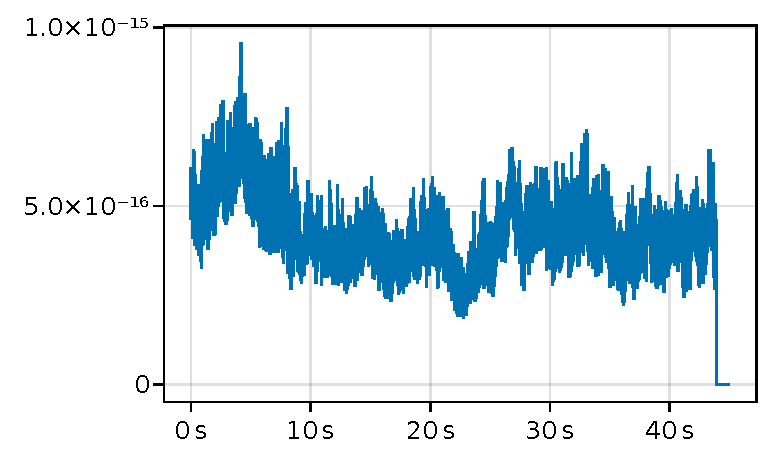
\includegraphics[width=\textwidth]{figures/slides-seq-parareal-ref.pdf}
      \end{columns}
      \end{minipage}
  \end{itemize}
\end{frame}

